\section{Introduction}
\label{sec:introduction}

% state the learning objective 
The objective of this laboratory assignment is to create a AC/DC Converter, a circuit that converts alternate current
into direct current, composed by an envelope detector, which includes a rectifier and a capacitor, and a voltage regulator which consists in a capacitor, a resistor and also a limiter. As seen in Figure \ref{fig:rc}, it was used a full wave bridge rectifier, and the limiter is composed by a group of 23 diodes in series.

\begin{figure}[h] \centering
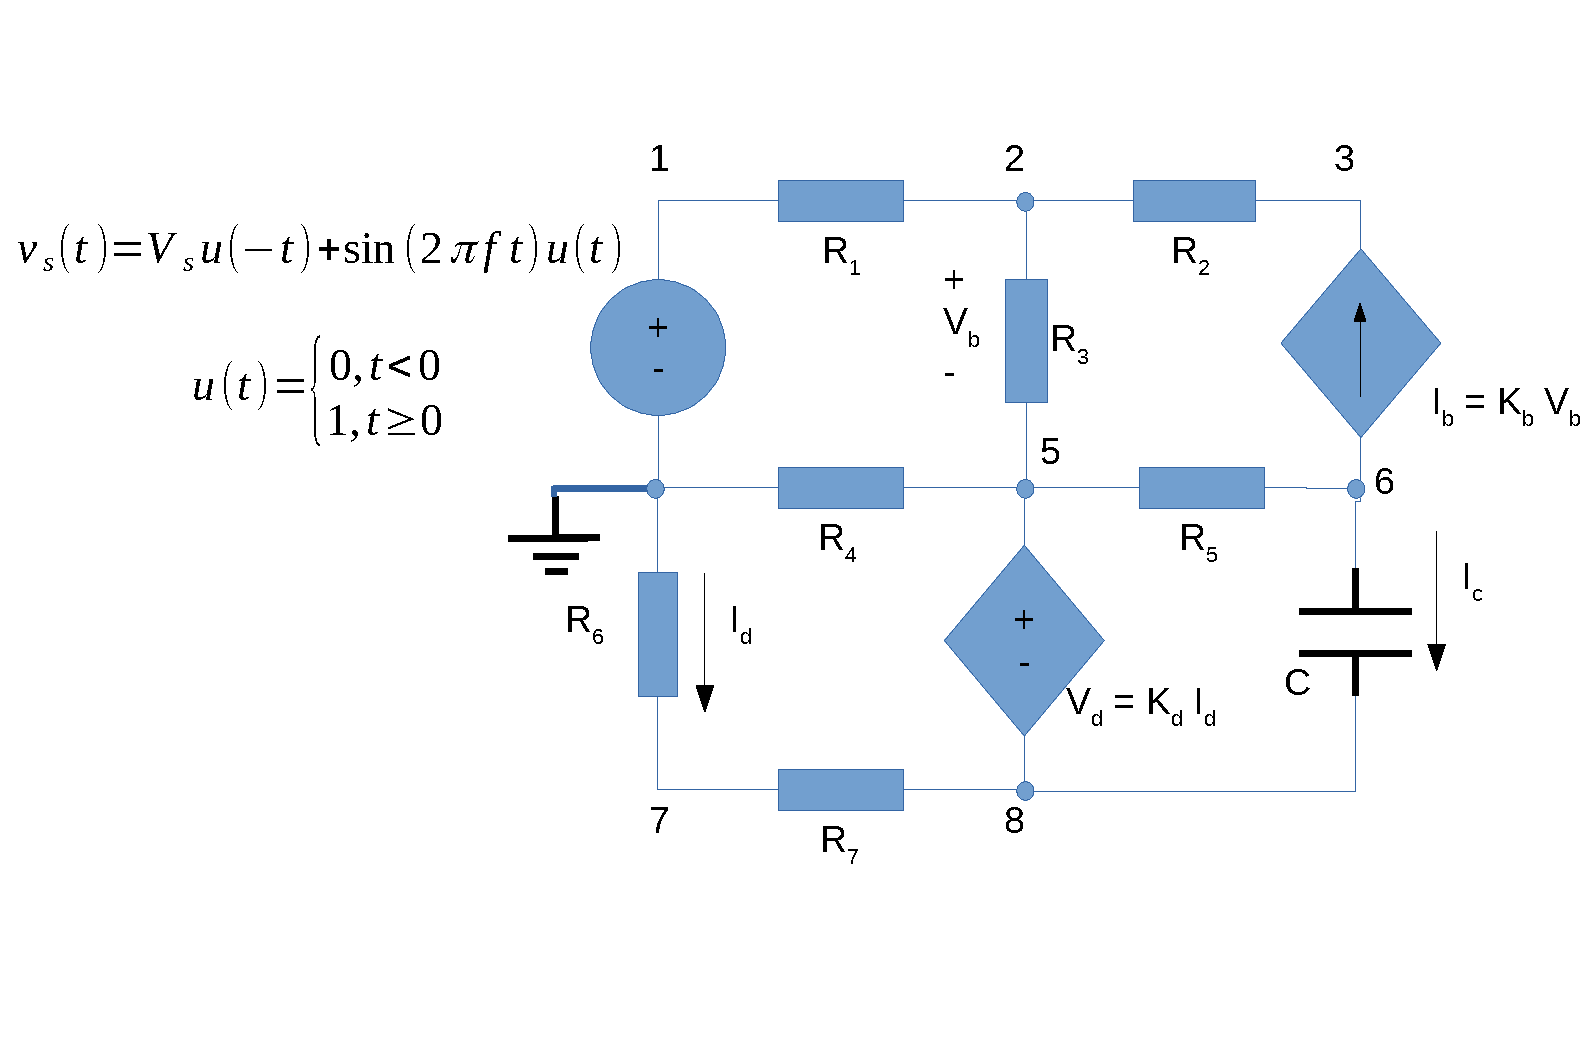
\includegraphics[width=0.8\linewidth]{rc.pdf}
\caption{The circuit under analysis}
\label{fig:rc}
\end{figure}

In Section \ref{sec:analysis1}, a theoretical analysis of the circuit is
presented, following a series of steps. In Section\ref{sec:simulation}, the circuit is analysed by
simulation, and the results are compared to the theoretical results obtained in
Section~\ref{sec:analysis}. The conclusions of this study are outlined in
Section~\ref{sec:conclusion}.





